\section{Game 2048}

2048 is a single-player stochastic game played on a $4 \times 4$ grid.
The objective of the original game is to reach a 2048-tile by moving and merging
the tiles on the board according to the rules below.
In an initial state, two tiles are randomly placed each with a number 2 (with probability $0.9$) or 4 (with probability $0.1$).
The player selects a direction (either up, right, down, or left), and then all tiles move in the selected direction.
When two tiles of the same number collide, they create a tile with the sum value, and the player gets the sum as the score.
The merges occur from the far side and newly created tiles do not merge again on the same move: moving to the right from \verb*|222 |, \verb*| 422| and \verb*|2222| results in
\verb*|  24|, \verb*|  44|, and \verb*|  44|, respectively.
Note that the player cannot select a direction in which the tiles do not move or merge.
After each move, a new tile appears randomly in an empty cell with number 2 (with probability $0.9$) or 4 (with probability $0.1$).
If the player cannot move the tiles in any direction, the game ends.

Fig.~\ref{fig:states-and-afterstates} depicts the process of the game.
Selecting right at the state $s_t$ in Fig.~\ref{fig:states-and-afterstates}, the tiles move to the right and
two 2-tiles and two 8-tiles merge, adding the score 4 + 16 = 20.
Then, a new tile appears to reach the next state $s_{t+1}$.

\begin{figure}
  \centering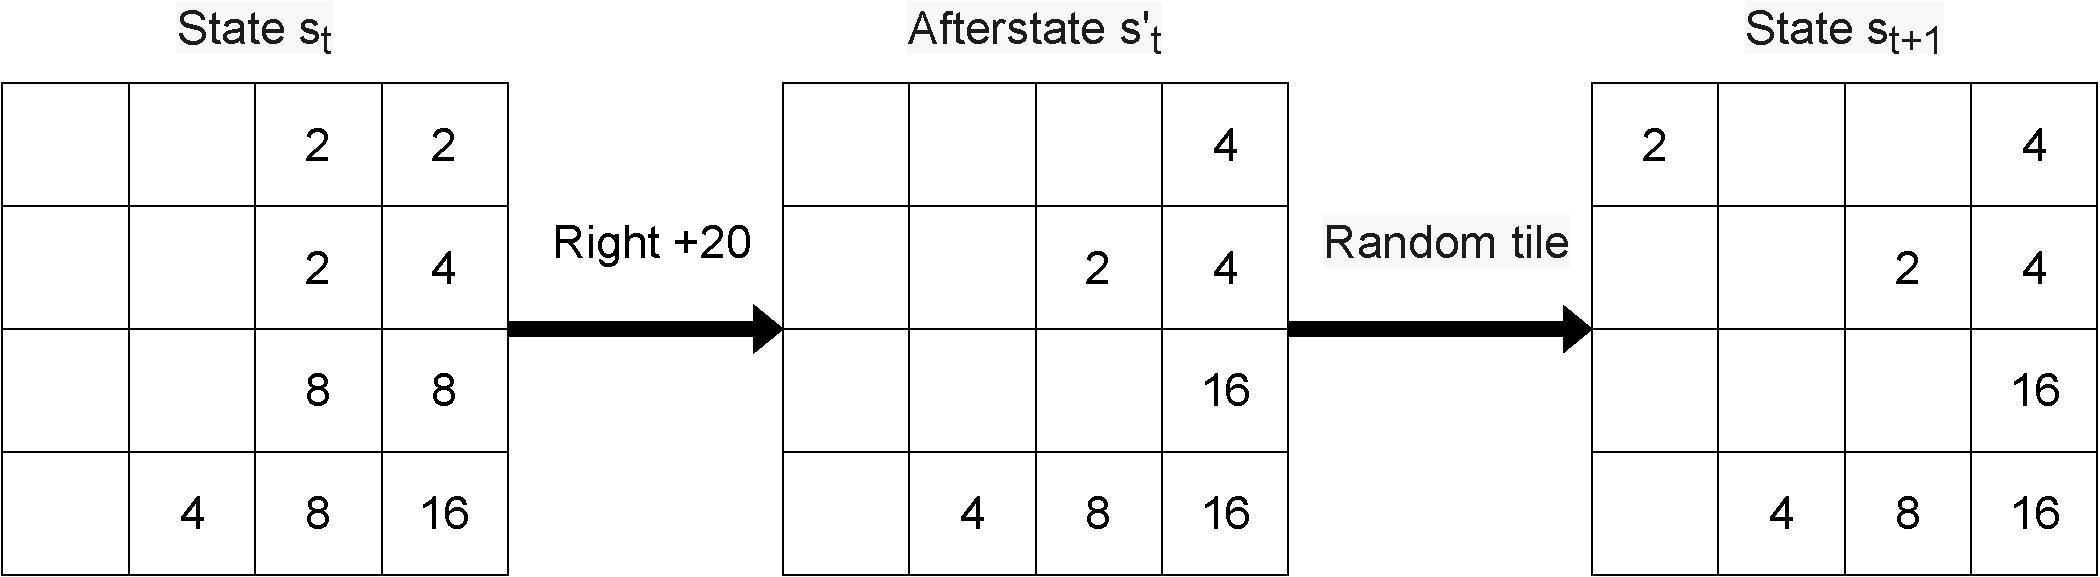
\includegraphics[width=.8\linewidth]{figures/state_afterstate.pdf}
 \caption{Process of the game 2048}
 \label{fig:states-and-afterstates}
\end{figure}

Since a turn in 2048 consists of two steps, we introduce the two notions, called \emph{state} and \emph{afterstate}~\cite{SzJa14}, as shown in Fig.~\ref{fig:states-and-afterstates}.
\begin{itemize}
 \item A \emph{state} $s_t$ is a board (and score) at which the player selects a move.
 \item An \emph{afterstate} $s'_t$ is a board (and score) after the slide-and-merge step and before a new tile appears.
\end{itemize}

For a better understanding of the performance of the players, Table~\ref{table:achievement} summarizes the common score achieved and the common number of moves needed when the player reaches a tile of a specific value.

\begin{table}
 \caption{Score and number of moves when a tile is first created}
\setlength{\doublerulesep}{.4pt}
 \label{table:achievement}
 \centering\begin{tabular}{lrrrrr}
\hline
\hline
  tile & \makebox[4em][r]{2048} & \makebox[4em][r]{4096} & \makebox[4em][r]{8192} & \makebox[4em][r]{16384} & \makebox[4em][r]{32768} \\
\hline
  score & 20\,000 & 44\,000 & 97\,000 & 210\,000 & 450\,000 \\
\hline
  moves &     950 & 1\,900 &  3\,800 & 7\,600 & 15\,200 \\
\hline
 \end{tabular}
\end{table}

% 図\ref{afterstate2048}は,初期局面から始まるゲームの流れにおいて,state,afterstate,progress を図示したものである.

